%!TEX root = thesis.tex

\chapter{Approach}
\label{ch:approach}
\todo{Short introduction. Describe idea. This builds on top of related work as combines minimax with rulebased}
\todo{Predictions: Use Move against most likely next enemy. No prediction switching (yet)}
\todo{Matchups only recalculated on new information.}
\section{Communication with Pokémon Showdown}
\label{sec:poke-env}
The communication with Pokémon Showdown is handled using the python library \textit{Poke-Env} ~\autocite{PokeEnv:Github}.
This library provides a lot of the core functionality needed, like accessing the current Pokémon in battle as well
as switch and move options. However, it does not provide functionality for damage calculation. We use the \textit{Pokémon
Damage Calculator} ~\autocite{Smogon:DamageCalc}, a node library written by the smogon-team for that. 
Communication between the two libraries is implemented by capturing stdout and stdin using the \textit{subprocess} python library.

\section{Gathering Information about the enemy Pokémon}
\label{sec:builds-randbats}
As mentioned in \ref{sec:showdown-randbats}, the same Pokémon can occur in various different builds, meaning the combination
of moves, abilities and items. Knowing the exact build is crucial for the decision-making process. Consider the following
example: 
\begin{itemize}
	\item \textbf{Player1} has an active \textit{Charizard} with \textit{Heavy-Duty Boots} and 150\ac{HP} remaining on the field.
	\item \textbf{Player2} has just sent out a \textit{Drapion} with 160\ac{HP} remaining.
	\item The \textit{Charizard} is faster but can not kill the enemy \textit{Drapion} in one turn as his move 
	\textit{Fire Blast} deals between 127 and 151 damage to the \textit{Drapion}. 
	\item Therefore, if \textbf{Player1} decides to attack, \textit{Drapion} is guaranteed to survive this turn
	and can attack \textit{Charizard} as well.
\end{itemize}
In this scenario, the optimal strategy for \textbf{Player1} depends heavily on the move set of the enemy \textit{Drapion}.
Possible moves for \textit{Drapion} are:
\begin{itemize}
	\item \textit{Aqua Tail}: A damaging \textit{Water}-type move
	\item \textit{Earthquake}: A damaging \textit{Ground}-type move
	\item \textit{Knock Off}: A damaging \textit{Dark}-type move
	\item \textit{Poison Jab}: A damaging \textit{Poison}-type move
	\item \textit{Swords Dance}: A move to raise the own \ac{ATK} by two stages
	\item \textit{Taunt}: A move that makes the afflicted Pokémon unable to use status moves
	\item \textit{Toxic Spikes}: A move that sets an entry hazard.
\end{itemize}
Hereby it is important to note that \textit{Drapion} only knows the move \textit{Aqua Tail}, if it knows four total 
damaging moves\footnote{This information was extracted from all possible \textit{Drapion} builds. Details on 
how these builds were obtained are covered in \ref{sec:build-imp-details}}. 
In the given scenario, \textbf{Player1} should switch out his \textit{Charizard} if the enemy
\textit{Drapion} knows the move \textit{Aqua Tail} as this attack would kill \textit{Charizard}. We can determine 
whether the enemy knows \textit{Aqua Tail} based on his item:
\begin{itemize}
	\item If \textit{Drapion} rolls two status moves, it will have the item \textit{Black Sludge} and therefore 
	doesn't know \textit{Aqua Tail}. Because \textit{Drapion} is already damaged, we know that it has this item
	if it healed 1/16\% of his max \ac{HP} in his last turn. 
	\item If \textit{Drapion} rolls one status move, it will have the item \textit{Life Orb}. If \textit{Drapion}
	already attacked, we know if it has a \textit{Life Orb} or not as this item causes it to lose 10\% of his
	maximum \ac{HP} after an attack.
	\item If \textit{Drapion} has neither \textit{Black Sludge} nor \textit{Life Orb}, it has to have a
	\textit{Choice Band} and as this item will only generate if the Pokémon knows four matching attacks,
	and therefore has to know the move \textit{Aqua Tail}.
\end{itemize}
Therefore, the player should switch out his \textit{Charizard} if the \textit{Drapion} has neither \textit{Black Sludge}
nor \textit{Life Orb} as then it is guaranteed to have a \textit{Choice Band}, knows \textit{Aqua Tail} and would therefore
be able to defeat \textit{Charizard}. In any other case, the \textbf{Player1} can safely kill \textit{Drapion} using his
active \textit{Charizard}.

\paragraph{Implementation details}
\label{sec:build-imp-details}
The first step to predicting enemy sets is to determine all possible sets and the likeliness of each individual set.
In order to achieve this, I wrote a script that starts a battle between an information gathering player and 
a random agent. In the next step, the script extracts all builds of all Pokémon and stores them. Then, it forfeits, 
and a new battle is started. Once enough battles are fought, the script will store the builds as well as how often
they appeared in text files, one file for each Pokémon. \\
In actual battles, if a new Pokémon enters the enemy side, we assume it to have the most likely build for its species. 
Once more information becomes available on items, moves and abilities, we rule-out non-matching builds and always
assume the enemy to have the remaining most likely build.

\section{Scoring the current game state}
\label{sec:scoring-state}
In order to not only rate the current board state, but also individual Pokémon, we implement the following scoring 
algorithm:
\begin{equation}
\label{eq:score-attack}
	score(e_{i, j}) = \text{Expected Damage that Pokémon } i \text{ will deal to Pokémon }j
\end{equation}
The expected damage is the damage dealt if both Pokémon behave optimal in the amount of turns that the bot looks into
the future. Section \ref{sec:determine-matchups} covers how the optimal moves are determined.
\begin{equation}
	value(i) = \sum_{j \in \text{Enemy Pokémon}} score(e_{i, j})
\end{equation}
Using this, we can also introduce a \textit{value} for each of our Pokémon where a higher value implies a more important
Pokémon. It is important to note that scores are determined independently of each other meaning that we do not take
into account damage taken by the attacker. This does imply that this metric does not determine how good the 
Pokémon is if it has to battle \textit{all} enemy Pokémon but rather against how many other Pokémon it \textit{could}
be used. This is done as the order in which a Pokémon battles multiple Pokémon plays a critical role. The reasoning
behind this as well as the determination of an optimal order is explained in section \ref{sec:defeat-phase}.
This metric also has multiple flaws because it only takes the damage dealt to the enemy into account, other important 
factors like damage received, healing, the availability of status moves and hazards is not considered. Using 
this rating, we can rank our team based on importance which is used in the switching routine described in 
section \ref{sec:stages-of-game}.

\section{Stages of the game}
\label{sec:stages-of-game}
We divide the game into two phases, the first one being the \textit{Discover}-Phase whereas the second phase is called
\textit{Defeat}-Phase. Our goal and therefore our play style, is different in both phases.
\paragraph{Discover Phase}
At the beginning of the game, we play safely until we know our opponent's entire team. In other words, we try to gather 
information about the enemy team while sacrificing as little \ac{HP} as possible. In this stage, we act according to
these rules:
\begin{enumerate}
	\item Kill the opponent if we are guaranteed to kill him this turn. This either leads to us defeating the 
	enemy Pokémon, or possibly new information if the enemy switches.
	\item Healing our Pokémon. If we have a healing move that will heal us more than the expected damage we receive
	this turn, and we are not at full \ac{HP} we will heal our Pokémon. Doing so will force the enemy to switch as
	we are otherwise gaining an advantage over him. \todo{Go into a bit more depth here?}
	\item If we have a hazard setting move available, we will use this move as they will help us in the \textit{Defeat}-Phase.
	Other beneficial side-conditions like \textit{Light Screen} will be set as well. 
	\item Using moves that inflict status to the opponent like \ac{BRN}.
\end{enumerate}
If none of these conditions apply, we decide whether to switch out our Pokémon or not. If our current Pokémon is a 
\textit{check} or \textit{counter} against the enemy Pokémon, we will not switch. Otherwise, we switch to a \textit{check},
or \textit{counter} if present. Next, we check if the current matchup is unfavorable. This applies, if the enemy
is expected to survive the current matchups for two turns longer than we do, meaning that our Pokémon would not be able
to defeat the enemy, if it was allowed to attack two additional times. If this is the case, we determine the next action
as follows: \\
We start by determining the \textit{score} of each of our Pokémon as described in formula \ref{eq:score-attack} and exclude our
two most valuable Pokémon from the next steps. This is done as we assume to depend heavily on these Pokémon to defeat
other enemies. Next up, we pick the Pokémon with the lowest \textit{score} that fulfills the following 
criteria:
\begin{itemize}
	\item The Pokémon has to survive for at least three turns against the enemy
	\item At least one of the following criteria apply:
	\begin{itemize}
		\item It is able to set a \textit{hazard} or other beneficial field effect that is not already present.
		\item It can inflict a status condition on the enemy.
	\end{itemize}
\end{itemize}
If no Pokémon matches these criteria, the Pokémon with the lowest score is picked instead.
Score is calculated as described in section \nameref{sec:scoring-state}. \\
In any other case, the currently active Pokémon will use the best move calculated in \ref{sec:determine-matchups}.

\paragraph{Defeat Phase}
\label{sec:defeat-phase}
\todo{Move tree to appendix. If the tree is to small printed (when on appendix): Smaller Example using TikZ.}
The \textit{Defeat}-Phase starts as soon as we know all enemy Pokémon. At the beginning of this stage, we have to create
a match plan for defeating the enemy. The main goal is to figure out which Pokémon to use against which enemies, especially
the best order to send them into battle. 
\begin{figure}[h]
	\centering
	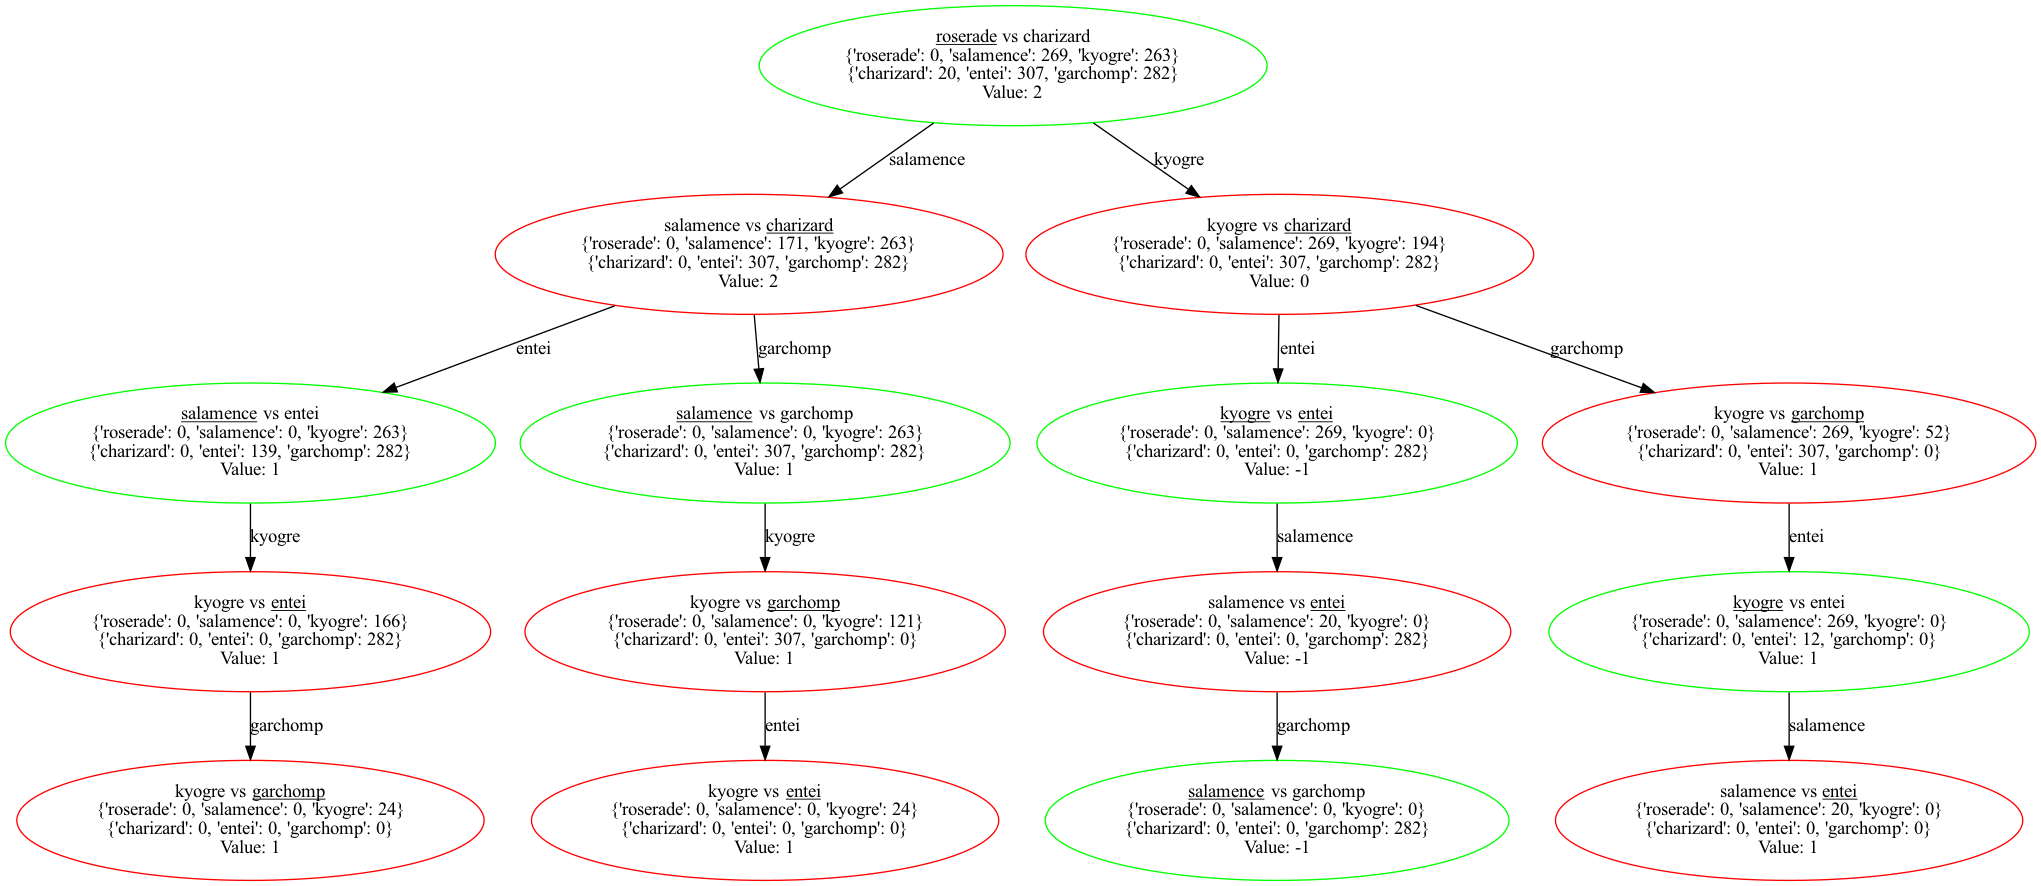
\includegraphics[width=1\textwidth]{images/MinMaxTree.png}
	\caption{Possible end game scenario}
	\label{fig:game-plan}
\end{figure}
Figure \ref{fig:game-plan} shows a possible end-game scenario. In this simple example, we assume both players to each
have three Pokémon with full \ac{HP} and no status conditions. Each circle represents two Pokémon battling each other.
Therefore, the circle in the top center indicates, that our \textit{Roserade} is currently fighting against the enemy
\textit{Charizard}. As \textit{Charizard} is a \textit{Fire}-type Pokémon which has a type advantage against his enemy,
our \textit{Roserade} will faint in this matchup, expressed by the underlined name. This means that Player 1 has to
switch in a new Pokémon. A green circle around a node illustrates that the first player has to make a turn as his 
Pokémon fainted, and a red circle marks a decision for Player 2. The first line below the names of the two opposing
Pokémon displays the amount of \ac{HP} the first team has left after this battle took place. As \textit{Roserade} fainted,
it has zero \ac{HP} left whereas the other two Pokémon in his team are still at full health. Below that, the remaining 
\ac{HP} of the second team is displayed. \textit{Charizard} is \textit{expected} to survive the battle with an 
\textit{expected} amount of 141 \ac{HP} remaining. Next, we have two possible options remaining, we can either send
\textit{Kyogre} or \textit{Azumarill} to defeat the enemy \textit{Charizard}. Taking a look at the leaves of the tree,
the \textit{value} of a leaf node is $-1$ if the enemy wins the battle and $1$ if we win the battle. 
The value of a non-leaf node is the sum of the \textit{values} of the children nodes. The \textit{value} of two means that we 
expect to win the battle. As a result of this, the best choice in our example scenario is to use \textit{Azumarill} to 
defeat the already damaged \textit{Charizard}. \\
\todo{Explain why MiniMax Tree is correct. Pokemon don't have expected items / moves!}

\section{Determining matchups}
\label{sec:determine-matchups}
In order to determine whether to attack or to switch, we need to determine how the optimal moves for a Pokémon against
another Pokémon are calculated. As stated before, the amount of possible combinations combined with the non-deterministic
nature of the game makes it unfeasible get the optimal move combination by simulating every possible combination of 
actions and reactions over the span of multiple turns. Therefore, we determine the optimal moves for a Pokémon using 
this simplified method: \\
We start by generating all possible move combinations for a Pokémon with a given length. Then, we simulate the outcome
of the battle. If the attacking Pokémon would use these moves in the defined order given the enemy would not do 
anything\footnote{The option of not doing anything in a turn does not exist in Pokémon, if possible, the player is always 
forced to either select a move or switch}. Here, we also take boosting, items, status effects and the possibly changing
field state into account.
The combination resulting in the lowest amount of turns until the enemy faints is selected. 
It is important to note that this is not necessarily the move that the bot will use in the next turn as in the 
\textit{Discover}-Phase healing, status and other beneficial effects are prioritized.

\section{Predictions}
\label{sec:predictions}
\todo{Explain predicting routine}
Predicting the next enemy action plays a huge role in competitive Pokémon. In many situations, it is very likely
that the opponent will switch to another Pokémon to avoid a bad matchup. For example, players often withdraw 
\textit{Fire}-type Pokémon if the opponent knows a \textit{Water}-type move as this will deal twice the amount of
damage due to the type multiplier discussed in section \ref{sec:types}. Therefore, players often choose to pick a move
countering the expected Pokémon the opponent will send out or even switch themselves in anticipation of an enemy
action. Our agent mimics this behavior in the following way: \\
The agent keeps track how often the opponent chose to withdraw his active Pokémon when it is checked and how often
he decided to stay in. In order to make the actions taken by the agent less predictable, \ac{RNG} is used on
favorable matchups to decide how to act. The chance that the agent predicts an enemy switch is zero if this is 
the first time that our Pokémon counters an enemy and otherwise as described in equation \ref{eq:prediction-chance}. 
\begin{equation}
\label{eq:prediction-chance}
	\text{Chance make a prediction} = 
	\frac
	{\text{\# The enemy switched when countered}}
	{\text{\# Total times the enemy was countered}}
\end{equation}
Currently, the agent assumes the enemy to switch in a random Pokémon that counters the active Pokémon and will then 
pick the move, that will yield to the best outcome for this matchup. Flaws and possible improvements to this
simple routine will be discussed in section \ref{par:predictions}. 
\section{Dynamaxing}
\label{sec:dynamaxing}
At the time of writing, \textit{Memezboi69} is the top ranked player on the Pokémon Showdown ladder. He described
the use of dynamaxing as very situation dependent as it can either be used offensive or defensive and proposed 
a simple rule set that can be build upon:
Dynamax if the current matchup is favorable, the entire enemy team is known and the active Pokémon has more than
70\% \ac{HP} remaining. In addition, the agent will dynamax if the current Pokémon is the last remaining Pokémon
with full \ac{HP}. \textit{Memezboi69} also laid out a more sophisticated rule set, which is described in
section \ref{par:eval-dynamx}, that can be applied in future iterations of the agent.